\documentclass[aspectratio=169, t, 8pt]{beamer}

%------configurando acentos-----------
\usepackage[utf8]{inputenc}
\usepackage[T1]{fontenc}
\usepackage[brazilian]{babel}
\usepackage{montserrat}
\usefonttheme[onlymath]{serif}
\usepackage{booktabs} % Tabelas elegantes sem linhas verticais
\usepackage{multirow}
\usepackage{array}
\usepackage[most]{tcolorbox}
\usepackage{graphicx}
\usepackage{xcolor}
\usepackage{colortbl}
\usepackage{ulem}
\usepackage{enumitem}

\DeclareMathOperator{\sen}{sen}
\DeclareMathOperator{\coss}{cos}
\DeclareMathOperator{\tg}{tg}
%-------Estilos Beamer---------------
\usetheme{metropolis}
%\usecolortheme{crane}
%\usefonttheme{serif}
\linespread{1.2}

% Personalização de Cores (Exemplo: Minimal Teal)
% Cores Base
\definecolor{BgCanvas}{HTML}{F9F9FB}      % Off-white muito suave
\definecolor{MainText}{HTML}{2B2D42}      % Grafite escuro para alta legibilidade
\definecolor{PrimaryAccent}{HTML}{15407f} % Azul poeira (Dusty Blue)

% Tons Pastéis para Destaques e Cards
\definecolor{PastelGreenBg}{HTML}{E8F0EC}  % Sálvia Claro (Sucesso / Destaque Positivo)
\definecolor{PastelGreenFg}{HTML}{2D5A44}

\definecolor{PastelCoralBg}{HTML}{FDEAE6}  % Coral Soft (Atenção / Problema / Alerta)
\definecolor{PastelCoralFg}{HTML}{7A3025}

\definecolor{PastelPurpleBg}{HTML}{F0EBF4} % Lavanda (Conceitos / Citações)
\definecolor{PastelPurpleFg}{HTML}{4A3E56}

\definecolor{PastelYellowBg}{HTML}{FFF4E6} % Areia / Manteiga (Notas / Dados Secundários)
\definecolor{PastelYellowFg}{HTML}{7A522A}

% --- CONFIGURAÇÕES DE TEMA BEAMER ---
%\usetheme{metropolis}

\setbeamertemplate{itemize item}{\textcolor{MainText}{$\bullet$}}
\setbeamertemplate{itemize subitem}{\textcolor{MainText}{\scriptsize$\circ$}}
\setbeamertemplate{itemize 3rditem}{\textcolor{MainText}{\tiny$\blacksquare$}}

\setbeamercolor{background canvas}{bg=BgCanvas}
\setbeamercolor{normal text}{fg=MainText}
\setbeamercolor{frametitle}{bg=PastelGreenFg, fg=BgCanvas}
\setbeamercolor{title}{fg=MainText}
\setbeamercolor{subtitle}{fg=PrimaryAccent}
\setbeamercolor{structure}{fg=PrimaryAccent}

% Remove a linha amarela padrão do Metropolis sob o título
\setbeamertemplate{title separator}{}
\setbeamertemplate{progress bar in section page}{}

% ==============================================================================
% PALETA DE CORES "AZUL MATEMÁTICO" (Inspirada na imagem)
% ==============================================================================
\definecolor{BgCream}{HTML}{FFFDFB}       % Fundo creme suave
\definecolor{TextDark}{HTML}{1A2530}      % Texto em castanho escuro elegante
\definecolor{PrimaryBlue}{HTML}{0F52BA}  % Laranja vibrante (Títulos e destaques)
\definecolor{DeepBlue}{HTML}{082846}     % Terracota queimado (Alertas)
\definecolor{SoftBlue}{HTML}{E6F0FA}     % Laranja bem suave (Fundo de blocos)

% =================================================
% CONFIGURAÇÃO DO TEMA METROPOLIS
% =================================================
% Cores do texto e fundo geral
\setbeamercolor{normal text}{fg=TextDark, bg=BgCream}
\setbeamercolor{alerted text}{fg=DeepBlue}
\setbeamercolor{example text}{fg=PrimaryBlue}

% Barra de título dos slides (Frametitle)
\setbeamercolor{frametitle}{fg=BgCream, bg=PrimaryBlue}

% Título principal da apresentação (Slide de Capa)
\setbeamercolor{titlelike}{fg=PrimaryBlue}
\setbeamercolor{subtitle}{fg=DeepBlue}

% Barra de progresso (Linha do Metropolis)
\setbeamercolor{progress bar}{fg=PrimaryBlue, bg=PrimaryBlue!20}

% Customização de Blocos (block, alertblock, exampleblock)
\setbeamercolor{block title}{fg=BgCream, bg=PrimaryBlue}
\setbeamercolor{block body}{fg=TextDark, bg=SoftBlue}

\setbeamercolor{block title alerted}{fg=BgCream, bg=DeepBlue}
\setbeamercolor{block body alerted}{fg=TextDark, bg=DeepBlue!15}


% --- ESTILOS DE CARDS PASTEL COM TCOLORBOX ---
\newtcolorbox{cardPrincipal}[1][]{
  colback=SoftBlue,
  colframe=DeepBlue,
  coltext=TextDark,
  arc=6pt,
  boxrule=0pt,
  left=12pt, right=12pt, top=10pt, bottom=10pt,
  fonttitle=\bfseries\small,
  #1
}

\newtcolorbox{cardcoral}[1][]{
  colback=PastelCoralBg,
  colframe=PastelCoralFg,
  coltext=PastelCoralFg,
  arc=6pt,
  boxrule=0pt,
  left=12pt, right=12pt, top=10pt, bottom=10pt,
  fonttitle=\bfseries\small,
  #1
}

\newtcolorbox{cardpurple}[1][]{
  colback=PastelPurpleBg,
  colframe=PastelPurpleFg,
  coltext=PastelPurpleFg,
  arc=6pt,
  boxrule=0pt,
  left=12pt, right=12pt, top=10pt, bottom=10pt,
  fonttitle=\bfseries\small,
  #1
}

\newtcolorbox{cardyellow}[1][]{
  colback=PastelYellowBg,
  colframe=PastelYellowFg,
  coltext=PastelYellowFg,
  arc=6pt,
  boxrule=0pt,
  left=12pt, right=12pt, top=10pt, bottom=10pt,
  fonttitle=\bfseries\small,
  #1
}

\graphicspath{{../../src/img/semana11/}}

%--------Dados do Documento
\title{ENEM: Listão}
\subtitle{}
\author{prof. Eduardo}
\institute{Pré-Universitário Oficina do Saber / UFF}

\date{\today}


%-------- Pacotes Matemática -------------
\usepackage{amsmath}
\usepackage{amsthm}
\usepackage{amsfonts}
\usepackage{amssymb}
\usepackage{xfrac}
\usepackage{thmtools}

\begin{document}

    \begin{frame} %capa
        \vspace*{\fill}
            
            \begin{columns}[c]
                \begin{column}{0.5\textwidth}
                    {\usebeamerfont{title}\usebeamercolor[fg]{title}\inserttitle}\vspace{0.2cm}
                    
                    {\usebeamerfont{subtitle}\usebeamercolor[fg]{subtitle}\insertsubtitle}\vspace{0.5cm}

                {\usebeamerfont{author}\insertauthor}\vspace{0.3cm}

                {\usebeamerfont{institute}\insertinstitute}\vspace{0.3cm}

                {\usebeamerfont{date}\insertdate}
            \end{column}
            
            
            \begin{column}{0.4\textwidth}
                \centering
                
\includegraphics[width=0.4\textwidth]{../logo_ofSaber.png}

                \vspace{.4cm}
                \vspace*{\fill}
        \begin{columns}[c]
            \begin{column}{.5\textwidth}
                \centering
\includegraphics[width=.5\textwidth]{../Proex02c.png}
            \end{column}
            \begin{column}{.5\textwidth}
                \centering
\includegraphics[width=0.4\textwidth]{../Logo_UFF.png}
            \end{column}
        \end{columns}
        \vspace*{\fill}
            \end{column}
        \end{columns}
    \vspace*{\fill}
    \end{frame}

    % \frame
        % {
        %     \usebackgroundtemplate{
        %     \includegraphics[width=\paperwidth]{segunda_capa_pitagoras.png}}
        %     \begin{frame}[plain]                
        %     \end{frame}
        % }

    \begin{frame}{Garante Nota}
        \begin{columns}[totalwidth=.9\textwidth, T]
            \begin{column}{\textwidth}
                \textcolor{black!65}{\bf Questão 138 (Caderno Amarelo/2024):} Uma empresa de engenharia foi contratada para realizar um serviço no valor de $\text{R\$} \;71.250,00$. Os sócios da empresa decidiram que $40\%$ desse valor seria destinado ao pagamento de três engenheiros que gerenciaram o serviço.
                
                O pagamento para cada um deles será feito de forma diretamente proporcional ao total de horas trabalhadas. O número de dias e o número de horas diárias trabalhadas pelos engenheiros foram, respectivamente:
            \end{column}
        \end{columns}

        \vspace{1em}

        \begin{columns}[totalwidth=.9\textwidth, T]
            \begin{column}{.4\textwidth}
                \begin{itemize}[label=$\bullet$]
                    \item engenheiro I: 4 dias, numa jornada de 5 horas e meia por dia;
                    \item engenheiro II: 5 dias, numa jornada de 4 horas por dia;
                    \item engenheiro III: 6 dias, numa jornada de 2 horas e meia por dia.
                \end{itemize}
            \end{column}
            \begin{column}{.45\textwidth}
                Qual a maior diferença, em real, entre os valores recebidos por esse serviço entre dois desses engenheiros?
                \begin{enumerate}[label=\alph*.), font=\bfseries]
                    \item 1000
                    \item 1500
                    \item 3500
                    \item 3800
                    \item 5250
                \end{enumerate}
            \end{column}
        \end{columns}
    \end{frame}

    \begin{frame}{Garante Nota}
        \begin{columns}[totalwidth=.9\textwidth]
            \begin{column}{\textwidth}
                 \textcolor{black!65}{\bf Questão 146 (Caderno Amarelo/2022):} Uma pessoa pretende instalar um kit de gás natural veicular (GNV) em seu carro. Na loja que escolheu para realizar a compra e instalação desse kit, havia cinco modelos de cilindro para armazenamento do gás, cujas capacidades, em metro cúbico, eram, respectivamente: 10, 14, 17, 21 e 25. O preço do cilindro é proporcional à sua capacidade. Esse carro rodará 30 km diariamente, 7 dias por semana, e o consumo do GNV é de $1\text{ m}^3$ a cada 13 km rodados. A pessoa escolherá o modelo de cilindro de menor preço e que garanta apenas um abastecimento semanal.

                 Nessas condições, qual será a capacidade, em metro cúbico, do cilindro escolhido por essa pessoa?
                
                \begin{enumerate}[label=\alph*.), font=\bfseries]
                    \item 10
                    \item 14
                    \item 17
                    \item 21
                    \item 25
                \end{enumerate}
            \end{column}
        \end{columns}
    \end{frame}

    \begin{frame}{Mediana}
        \begin{columns}[totalwidth=.9\textwidth]
            \begin{column}{\textwidth}
                 \textcolor{black!65}{\bf Questão 137 (Caderno Amarelo/2024):} A umidade relativa do ar é um dos indicadores utilizados na meteorologia para fazer previsões sobre o clima. O quadro apresenta as médias mensais, em porcentagem, da umidade relativa do ar em um período de seis meses consecutivos em uma cidade.

                \begin{figure}
                    \centering
                    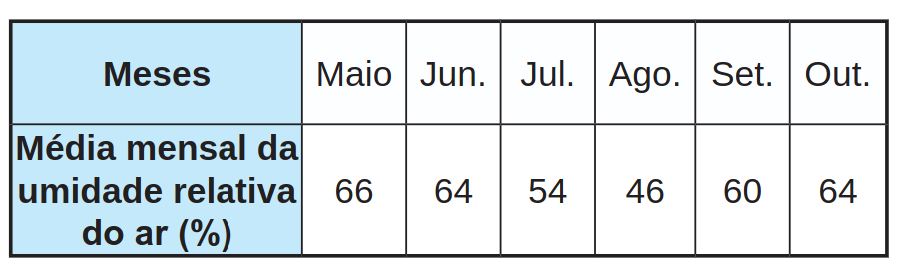
\includegraphics[width=.6\textwidth]{tabela_umidade.png}
                \end{figure}

                 Nessa cidade, a mediana desses dados, em porcentagem, da umidade relativa do ar no período considerado foi
                
                \begin{enumerate}[label=\alph*.), font=\bfseries]
                    \item 56
                    \item 58
                    \item 59
                    \item 60
                    \item 62
                \end{enumerate}
            \end{column}
        \end{columns}
    \end{frame}


    \begin{frame}{Media}
        \begin{columns}[totalwidth=.9\textwidth]
            \begin{column}{\textwidth}
                 \textcolor{black!65}{\bf Questão 164 (Caderno Amarelo/2024):} Ao calcular a média de suas notas em 4 provas, um estudante dividiu, por engano, a soma das notas por 5. Com isso, a média obtida foi 1 unidade menor do que deveria ser, caso fosse calculada corretamente.

                 O valor correto da média das notas desse estudante é
                
                \begin{enumerate}[label=\alph*.), font=\bfseries]
                    \item 4
                    \item 5
                    \item 6
                    \item 19
                    \item 21
                \end{enumerate}
            \end{column}
        \end{columns}
    \end{frame}

    \begin{frame}{Funções}
        \begin{columns}[totalwidth=.9\textwidth]
            \begin{column}{\textwidth}
                \textcolor{black!65}{\bf Questão 179 (Caderno Amarelo/2024):} Uma caneca com água fervendo é retirada de um forno de micro-ondas. A temperatura $T$, em grau Celsius, da caneca, em função do tempo $t$, em minuto, pode ser modelada pela função $T(t) = a + 80\ b^t$, representada no gráfico a seguir.
            \end{column}
        \end{columns}

        \vspace{1.6em}
        
        \begin{columns}[totalwidth=.9\textwidth, T]
            \begin{column}{.5\textwidth}
                \begin{figure}
                    \centering
                    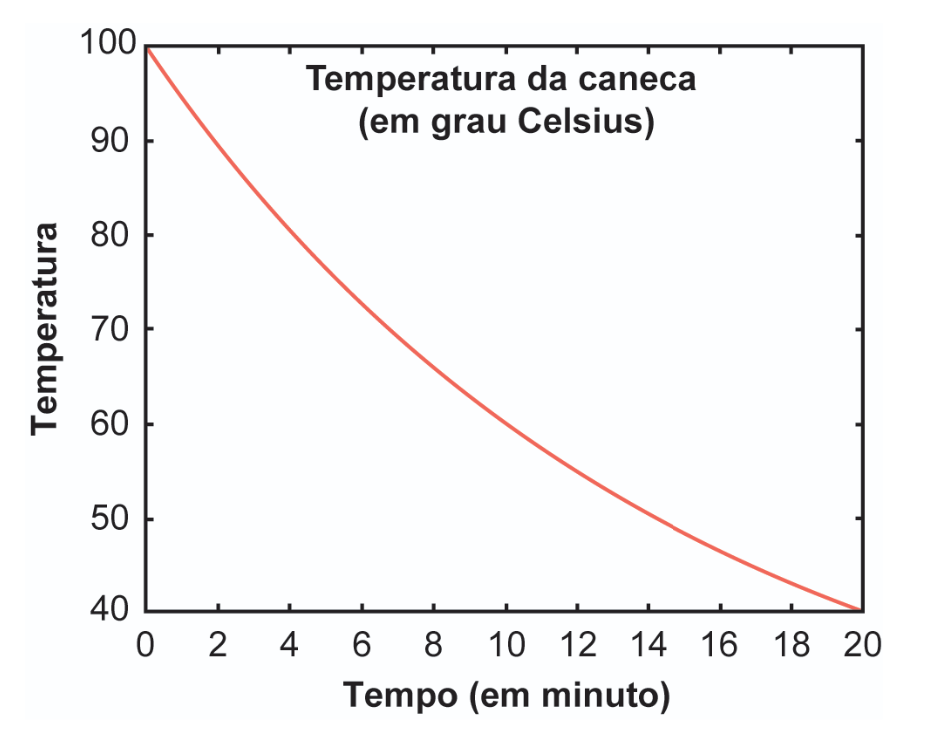
\includegraphics[width=\textwidth]{grafico_funcao_caneca.png}
                \end{figure}
            \end{column}

            \begin{column}{.4\textwidth}
                Os valores das constantes $a$ e $b$ são:

                \vspace{1em}

                \begin{enumerate}[label=\alph*.), font=\bfseries]
                    \item $\displaystyle a=20; \; b=\log{(0,5)}$
                    \item $\displaystyle a=100; \; b=0,5$
                    \item $\displaystyle a=20; \; b=(0,5)^{\frac{1}{10}}$
                    \item $\displaystyle a=20; \; b=\frac{40^{\frac{1}{10}}}{80}$
                    \item $\displaystyle a=20; \; b=40$
                \end{enumerate}
            \end{column}
        \end{columns}
    \end{frame}

    \begin{frame}{Funções}
        \begin{columns}[totalwidth=.9\textwidth]
            \begin{column}{\textwidth}
                \textcolor{black!65}{\bf Questão 171 (Caderno Amarelo/2025):} Quatro amigos, cada um com 100 moedas, criaram um jogo, no qual cada um assume uma das quatro posições, 1, 2, 3 ou 4, indicadas na figura, e nela permanece até o final. O desenvolvimento do jogo se dá em rodadas e, em todas elas, cada jogador transfere e recebe uma quantidade de moedas, da seguinte maneira:
            \end{column}
        \end{columns}
        \begin{columns}[totalwidth=\textwidth, T]
            \begin{column}{.45\textwidth}
                \begin{figure}
                    \centering
                    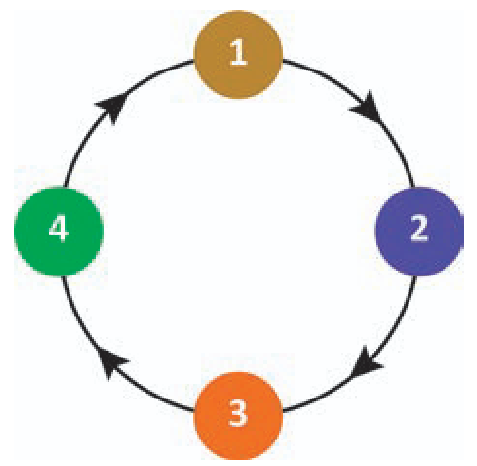
\includegraphics[width=.6\textwidth]{esquema_jogadas.png}
                \end{figure}

            \begin{itemize}[label=$\bullet$]
                    \item o jogador na posição 1 transfere 1 moeda para o jogador na posição 2;
                    \item o jogador na posição 2 transfere 2 moedas para o jogador na posição 3;
            \end{itemize}
                
            \end{column}
            \begin{column}{.5\textwidth}
                \begin{itemize}[label=$\bullet$]
                    \item o jogador na posição 3 transfere 3 moedas para o jogador na posição 4;
                    \item o jogador na posição 4 transfere 4 moedas para o jogador na posição 1, completando a rodada. 
                \end{itemize}
                Ao final da rodada $n$, qual é a expressão algébrica que representa o número de moedas do jogador na posição 1?

                \vspace{1em}

                \begin{tabular}{c c c}
                    \textbf{a.)} $103 + 4n$ & \textbf{b.)} $103 + 3n$ & \textbf{c.)} $100 + 4n$\\
                    \textbf{d.)} $100 + 3n$& \textbf{e.)} $99 + 4n$
                \end{tabular}
            \end{column}
        \end{columns}
    \end{frame}


    \begin{frame}{Geometria}
        \begin{columns}[totalwidth=.9\textwidth]
            \begin{column}{\textwidth}
                \textcolor{black!65}{\bf Questão 168 (Caderno Amarelo/2025):} A figura ilustra o projeto visual para confecção de uma medalha comemorativa, com a forma de um cilindro circular reto, de diâmetro 6 cm e espessura 3 mm.

                A figura $ABCD$ tem a forma de um quadrado e é a base de um prisma que atravessa toda a medalha. A região da medalha externa a esse prisma será cunhada em ouro. Pretende-se cunhar 100 dessas medalhas.
            \end{column}
        \end{columns}

        \vspace{1.5em}

        \begin{columns}[totalwidth=.9\textwidth, T]
                \begin{column}{.48\textwidth}
                    \begin{figure}
                        \centering
                        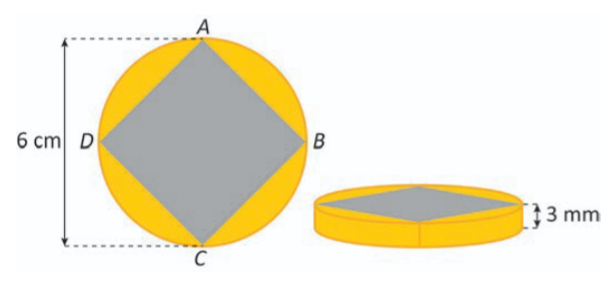
\includegraphics[width=.8\textwidth]{medalha.png}
                    \end{figure}

                    Considere 3,1 como valor aproximado para $\pi$. 
                \end{column}
                \begin{column}{.48\textwidth}
                    Qual é o volume de ouro, em centímetro cúbico, necessário para a confecção dessas medalhas?

                    \begin{enumerate}[label=\alph*.), font=\bfseries]
                        \item 288
                        \item 297
                        \item 567
                        \item 990
                        \item 1.134
                    \end{enumerate}
                \end{column}
            \end{columns}
    \end{frame}

    \begin{frame}{Geometria}
        \begin{columns}[totalwidth=.9\textwidth]
            \begin{column}{\textwidth}
                \textcolor{black!65}{\bf Questão 151 (Caderno Amarelo/2024):} Uma indústria faz uma parceria com uma distribuidora de sucos para lançar no mercado dois tipos de embalagens. Para a fabricação dessas embalagens, a indústria dispõe de folhas de alumínio retangulares, de dimensões 10 cm por 20 cm. Cada uma dessas folhas é utilizada para formar a superfície lateral da embalagem, em formato de cilindro circular reto, que posteriormente recebe fundo e tampa circulares. A figura ilustra, dependendo de qual das duas extensões será utilizada como altura, as duas opções para formar a possível embalagem.
            \end{column}
        \end{columns}

        \vspace{1.3em}

        \begin{columns}[totalwidth=.9\textwidth, T]
            \begin{column}{.4\textwidth}
                \begin{figure}
                    \centering
                    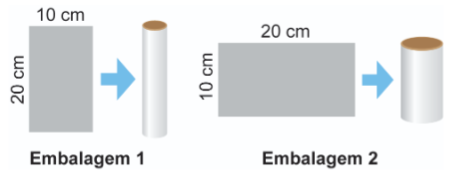
\includegraphics[width=\textwidth]{embalagens.png}
                \end{figure}
            \end{column}

            \hspace{.04\textwidth}

            \begin{column}{.55\textwidth}
                Dentre essas duas embalagens, a de maior capacidade apresentará volume, em centímetro cúbico, igual a
                
                \begin{enumerate}[label=\alph*.), font=\bfseries]
                    \item $4000\pi$
                    \item $2000\pi$
                    \item $\displaystyle \frac{4000}{\pi}$
                    \item $\displaystyle \frac{1000}{\pi}$
                    \item $\displaystyle \frac{500}{\pi}$
                \end{enumerate}
            \end{column}
        \end{columns}
    \end{frame}

    \begin{frame}{Probabilidade}
        \begin{columns}[totalwidth=.9\textwidth]
            \begin{column}{\textwidth}
                {\textcolor{black!65}{\bf Questão 161 (Caderno Amarelo/2024):}} Uma empresa tem 400 funcionários, distribuídos em três setores: administrativo, logística e produção. O gráfico apresenta a distribuição quantitativa desses funcionários, por setor e por faixa etária. Uma viagem de férias será sorteada entre esses funcionários, de forma que todos terão igual probabilidade de serem sorteados.

                A maior probabilidade é que o funcionário sorteado esteja na faixa etária
            \end{column}
        \end{columns}

        \vspace{1.em}

        \begin{columns}[totalwidth=.9\textwidth,T]
            \begin{column}{.25\textwidth}
                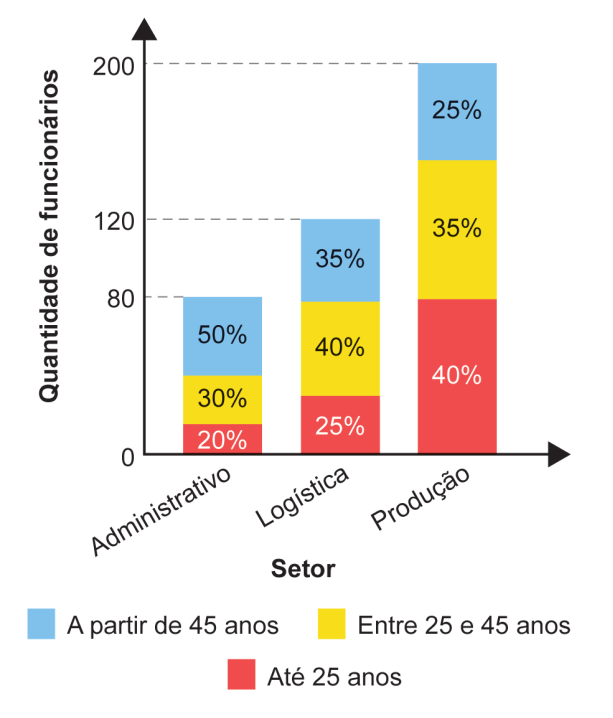
\includegraphics[width=\textwidth]{quetao161.png}
            \end{column}
            \begin{column}{.75\textwidth}
                \begin{enumerate}[label=\alph*.), font=\bfseries]
                    \item entre 25 e 45 anos, pois é a faixa etária com maior quantidade de funcionários.
                    \item entre 25 e 45 anos, pois é a única faixa etária cujas porcentagens são maiores do que as porcentagens mínimas de cada setor.
                    \item até 25 anos, pois é a única faixa etária cujos percentuais associados aos setores aumentam com o aumento da quantidade de funcionários por setor.
                    \item até 25 anos, pois é a faixa etária que apresenta maior quantidade de funcionários no setor de produção, que é o setor que emprega metade dos funcionários dessa empresa.
                    \item a partir de 45 anos, pois a soma das porcentagens associadas a essa faixa etária é 110\%, que é maior do que as respectivas somas associadas às outras faixas etárias, que são 105\% e 85\%.
                \end{enumerate}
            \end{column}
        \end{columns}
    \end{frame}

    \begin{frame}{Probabilidade}
        \begin{columns}[totalwidth=.9\textwidth]
            \begin{column}{\textwidth}
                {\textcolor{black!65}{\bf Questão 169 (Caderno Amarelo/2025):}} Três dados cúbicos, com faces numeradas de 1 a 6, foram utilizados em um jogo. Artur escolheu dois dados, e João ficou com o terceiro. O jogo consiste em ambos lançarem seus dados, observarem os números nas faces voltadas para cima e compararem o maior número obtido por Artur com o número obtido por João. Vence o jogador que obtiver o maior número. Em caso de empate, a vitória é de João.
                
                O jogador que tem a maior probabilidade de vitória é

                \vspace{1em}

                {
                \raggedright
                \begin{enumerate}[label=\alph*.), font=\bfseries]
                    \item Artur, com probabilidade de $\displaystyle \frac{2}{3}$\vspace{0.8em}
                    \item João, com probabilidade de $\displaystyle \frac{4}{9}$\vspace{0.8em}
                    \item Artur, com probabilidade de $\displaystyle \frac{91}{216}$\vspace{0.8em}
                    \item João, com probabilidade de $\displaystyle \frac{91}{216}$\vspace{0.8em}
                    \item Artur, com probabilidade de $\displaystyle \frac{125}{216}$  \vspace{0.8em}
                \end{enumerate}
                }
            \end{column}
        \end{columns}
    \end{frame}
\end{document}